\chapter{Diagrammes d'architecture}

Cette section contient les diagrammes d'architecture du projet. Cette section est divisée en deux parties, la première se concentre sur le site web tendit que la seconde se concentre sur le web service qui sera utilisé par les terminaux mobiles.

\newpage
\section{Le site web}

\newpage
\section{Le web service}
Les deux applications mobiles (Android et iOS) utiliseront la bibliothèque XZing \footnote{Lien vers le site web : \href{http://code.google.com/p/zxing/}{http://code.google.com/p/zxing/}} sous licence Apache 2.0.
Cette biliothèque permet de décoder un QRCode à partir d'une photo prise depuis un smartphone.

Pour l'interaction entre l'application et les terminaux mobiles, nous utiliserons la fonctionnalité de CakePHP pour créer des webservices capables de gérer un flux de données sous forme XML.
L'application contiendra donc un controleur qui servira des requêtes demandant des informations sur identifiant de matériel.

\begin{figure}[H]
	\begin{center}\fbox{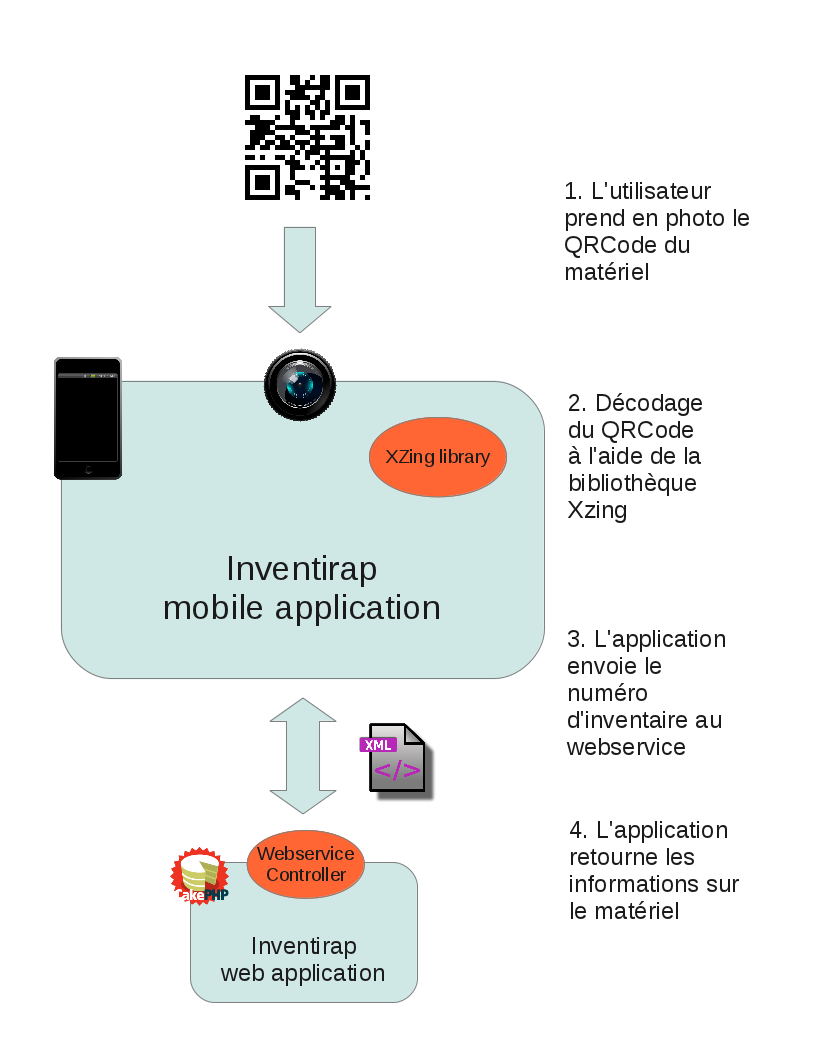
\includegraphics[]{images/webservice_schema.png}}\end{center}
	\caption{Schéma générale du webservice}
\end{figure}

\begin{figure}[H]
	\begin{center}\fbox{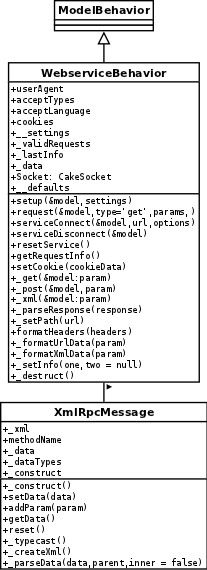
\includegraphics[]{images/webserviceController.png}}\end{center}
	\caption{Description des classes utiles au webservice}
\end{figure}
